\chapter{Quantum-dot cellular automata}

\graphicspath{{../gfx/chapter01/}}

\begin{figure}
  \center
  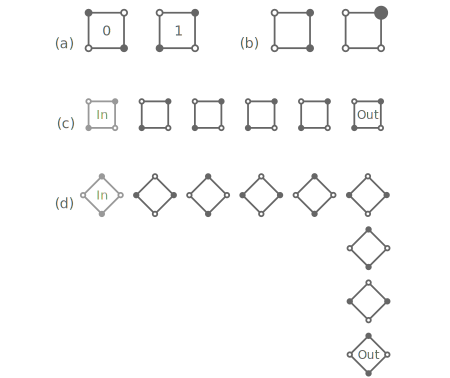
\includegraphics{intro_qca}
  \caption{\ldots}
  \label{fig:intro_qca}
\end{figure}

Lent et al.\ introduced the concept of quantum-dot cellular automata as an
alternative computing paradigm in 1993 \cite{lent1993quantum}. Thus the aim was
a novel physical scheme to build digital circuits that would overcome some of
the limitations of CMOS technology, promising potentially lower power
consumption, higher device density, and faster clocking. As the name alludes to,
quantum-dot cellular automata (QCA) is built from quantum-dots which are grouped
together in cells. Figure~\ref{fig:intro_qca}(a) shows a basic QCA cell. Four
quantum dots are arranged on the corners of a square. The dots are idealized as
perfectly localized single orbitals on a perfectly decoupled non-intrusive
medium. Therefore, each dot can be occupied by up to two electrons. In the QCA
scheme, however, each cell is occupied by only two electrons in total. The cell
is quarter-filled. The electrons tunnel between different dots in a cell, but
the dominant energy scale is set by the Coulomb repulsion between the particles.
Simply by virtue of the Coulomb repulsion, and ignoring the comparatively small
tunnelling for now, the diagonal states, Fig.~\ref{fig:intro_qca}(a), are the
two energetically preferred electron configurations. In comparison, edge states
or doubly occupied quantum dots are unfavourable higher energy states,
Fig.~\ref{fig:intro_qca}(b). A priori the two diagonal states are energetically
degenerate, but this degeneracy can be lifted by introducing an external Coulomb
potential, for example a second nearby QCA cell. Then these two states can be
identified with logic 0 and 1, as indicated in the figure.

A single cell by itself is, of course, not very interesting. Thus, multiple
cells can be positioned next to each other, for example as a straight line of
cells, Fig.\ref{fig:intro_qca}(c). The approach now again assumes that Coulomb
is the driving force and that electron tunnelling between cells is very small
and ideally zero. For a straight line of cells, these long-ranging, unscreened
Coulomb forces will tend to align the electron configurations of adjacent cells.
If the first cell is in logic state 1 then the second cell will also prefer
logic state 1 and so will in turn all the other cells in the line. The situation
is the same for logic state 0. Therefore, a straight line of cells is similar to
a wire not only in geometry, but also in functionality: It transmits a digital
signal. The same is true, with slight modifications, for a diagonal line of
cells --- cells rotated by $45^{\circ}$---, Fig.~\ref{fig:intro_qca}(d). In this
case the signal alternates from cell to cell, that is, logic 1 will follow logic
0 which followed from logic 0, and this again is simply by virtue of the
dominant Coulomb interactions between electrons on different cells. By using an
even number of cells the diagonal line of cells works as a wire just as well as
a straight line of cells. The pictogram also demonstrates a $90^{\circ}$ for the
diagonal line of cells which our newly gained intuition for these Coulomb-driven
systems expects to pose no problem for signal transmission.

The main idea of the QCA approach becomes apparent: Ideally bistable cells
interact with each other solely by Coulomb repulsion. By arranging the cells in
clever geometries we can realize interesting functionalities. The idea as such
is quite general and does not strictly rely on the two-electron-four-dot cell
introduced above. Indeed, a number of variations exist, such as
one-electron-two-dot cells, interacting via dipole fields instead of qudrupole
fields as for the conventional cells, or four-dot cells with six electrons---two
holes---instead of two electrons. Even the interaction need not be Coulombic.
For example, magnetic QCA schemes have been explored. While QCA carries
``quantum'' in its name and is sought to be implemented at the nanoscale, the
approach operates close to the classical limit. The Coulomb interaction is
absolutely dominating with the tunnelling of electrons a small perturbation,
which nonetheless drives the system's dynamics. The approach is insensitive and
in fact ignores the spin degree of freedom. Let us finally note that QCA is a
not a cellular automata in a strict mathematical sense, but only by analogy to
the idea of interacting cells.

One clever geometrical cell arrangement is the majority gate,
Fig.~\ref{fig:intro_qca}(e). The gate has three inputs which ``vote'' on the
central cell. The majority wins and sets the single output. The device is
commonly operated with one fixed input, for example $I_3 \doteq 0$ or $I_3
\doteq 1$. In the first case, $I_3 \doteq 0$, the device functions as an AND
gate for the remaining two inputs, $O = I_1 \land I_2$. In the second case, $I_3
\doteq 1$, it is an OR gate with $O = I_1 \lor I_2$. Now, the only missing piece
for Boolean algebra is negation, $O = \lnot I$. We had already seen that simply
arranging cells at an $45^{\circ}$ angle as in the diagonal line of cells above
negates the signal from cell to cell. The inverter, Fig.~\ref{fig:intro_qca}(f)
recasts this idea into a more robust layout. With that we have, at least in
principle, all the necessary building blocks for Boolean algebra and thus
digital circuitry.

Conceptually, it is most elegant to set the inputs to a QCA circuit via driver
cells --- cells that resemble the QCA cell in form, but are made up from static
point charges instead of quantum dots. These static charges are thought to be
manipulatable to vary the input smoothly from the logic 0 to the logic 1 state.
In figure~\ref{fig:intro_qca} these driver cells are represented in light grey.
Of course, in practice such driver cells would be difficult if not impossible to
implement and the input would more likely be set by leads that provide the
necessary perturbative electrostatic field. The output of a QCA device can be
directly read from its output cells. In practical implementations this will
require a non-trivial charge probing apparatus.

Changing the input for a QCA device throws the system into an excited,
non-equilibrium state. The system will then dissipatively propagate to its new
ground state. For the given inputs, this ground state corresponds to the
solution of the computational problem the circuit is designed to solve. Let us
emphasize this: In QCA, the computational solution maps directly to the physical
ground state! At all times during performing a computation, the system is
relatively close to its ground state. Only a few charges move locally, in each
cell. QCA is a truly current-free approach and consequently inherently
low-power, especially when compared with CMOS technology. But the operation
close to the ground state also raises concerns for the operational temperature
for these devices. It is clear that for applications we would want to engineer
the system so that the energy gap between the ground state and the low-lying
excited states far exceeds room temperature.

It is difficult to derive general expectations for the clocking speed of QCA
circuits. The switching speed of a majority gate, for example, will greatly
depend on the system's parameters, but particularly on the nature of the
dissipative coupling of the circuit to its environment. A small dissipative
coupling will have the output polarization oscillating before it eventually
settles to its correct value. A very dissipative system in contrast might get
stuck in meta-stable states. Different material systems provide different
dissipative channels and modelling them quantitatively or even qualitatively
correctly is very challenging.

QCA circuits consist of wires, gates, and other structures arranged on a
two-dimensional surface---very similar to conventional electronics devices.
However, the structures themselves are quasi-one-dimensional and this poses a
challenge for building large-scale QCA circuits. A good example is a single long
wire, which is truly one-dimensional. Generally, a one-dimensional system cannot
be ordered in the thermodynamic limit except at zero temperature. Therefore, the
finite-temperature infinitely long wire will always have at least two different
domains, logic 0 and logic 1 (assuming perfectly bistable cells for simplicity),
and thus not be able to transmit a signal. When we think about switching the
input for the wire, we think of the information being propagated as a charge
density wave throughout the wire, or, equivalently, as propagating the domain
boundary between logic 0 and logic 1. This domain boundary incurs an energy cost
that the system seeks to minimize. For an increasingly longer wire, however, the
gain in entropy for moving the domain boundary freely throughout the wire ($S
\sim \log N$, $N$ the number of cells) soon exceeds the loss in energy, which is
reflected by the free energy of the system, $A = U - T S$. Consequently, the gap
between the first excited state and the ground state and the desired operational
temperature will determine the maximum system size.

To address this scaling problem we partition large circuits into smaller units. 
Each unit can be turned ``on'' and ``off'' separately: Individual gates allow to
control the electrostatic potential for each unit, effectively raising and
lowering the tunnelling barriers between quantum dots and thus allowing to
freeze or delocalize the electrons. A unit with \emph{frozen} electrons can
serve as the input for a unit with more \emph{active} charge carriers, which
works like a regular QCA circuit. A unit with completely \emph{delocalized}
electrons, in contrast, will not influence adjacent units. By putting each unit
through the three phases \emph{delocalized}, \emph{active}, and \emph{frozen}
and synchronizing adjacent units appropriately, we can control the
information flow through the system very nicely, as illustrated in Fig.~TODO.
Therefore, by partition the circuit and introducing a clocking scheme we not
only handle the scaling problem, but also arrive at a pipelining architecture
that greatly improves the control over information flow in the system. Of
course, in practice the QCA circuit units cannot be too small as they must be
individually addressable. Gates which turn QCA units ``on'' and ``off'' also
provide another potential benefit. We are able to control how
and especially how fast the gate voltage is changed and should be able to tune
it with respect to the inherent time-scales of the QCA system, which are set by
the system's parameters and the dissipative coupling to its environment. This
should allow a better control over the dynamics of the switching process.

\begin{figure}
  \center
  \includegraphics{silicon}
  \caption{\ldots}
  \label{fig:silicon}
\end{figure}

% Silicon system

Our objective is the general, not implementation-specific characterization of
the QCA approach. Even so it is still important to consider concrete
experimental realizations, not only as a motivation for our work, but also to
put our modelling and results into context. One of the most promising and recent
experimental implementations of QCA is based on atomic silicon quantum dots and
we will therefore use them as our experimental reference. Atomic silicon quantum
dots were first demonstrated as a possible QCA implementation by Wolkow et~al.\
in 2009, when the group realized one single QCA cell. Fig.~\ref{fig:silicon}(a)
shows a scanning tunnelling microscope (STM) image of this cell. Since then
impressive advances have been made both in the understanding of the electronic
properties of these quantum dots as well as in the precise fabrication of larger
QCA structures. With atomic-scale feature sizes this experimental system
promises room temperature operation, while at the same time tapping into the
established and highly-sophisticated silicon technology. Being based on silicon
should also ease integration with existing CMOS circuitry.

Atomic silicon quantum dots are \emph{dangling bonds} on a hydrogen-terminated
silicon $(100)$ surface. Atoms on a $(100)$ silicon surface have two unsatisfied
bonds.  Pairs of surface atoms form dimers, satisfying one bond. The remaining
bond is satisfied by passivating the surface with hydrogen.
Fig.~\ref{fig:silicon}(c) shows a STM image of the reconstructed silicon
surface, where the dimer rows are clearly visible and the dimensions are
indicated. By applying a relatively large current through the STM tip,
individual hydrogen atoms can be removed, with atomic precision. This leaves a
\emph{dangling bond} (DB) which acts as a quantum dot: Energetically, electrons
on the DB orbital sit in the silicon band gap (see Fig.~\ref{fig:silicon}(b))
and are therefore decoupled from the silicon substrate. Chemically, DBs have
proven to be surprisingly robust with respect to environmental molecules. From
\emph{ab initio} calculations it is known that the $sp^3$ DB orbital extends
predominantly into the bulk and only a little into the vacuum. The orbital's
lateral extent is on the order of $1nm$ and therefore spans multiple silicon
lattice atoms. Due to the orbital overlap, closely spaced DBs are
tunnel-coupled. The neutral DB consists of the positive silicon ion and one
electron. In the experimentally common strongly n-doped system, the DB accepts
one more electron and is therefore $-1e$ negatively charged.  Conversely, in a
p-doped sytem the DB will donate its electron and become $+1e$ positively
charged. The Coulomb repulsion between negatively charged DBs can be used to
adjust the filling of DB assemblies simply by the DBs' positions. For example,
on a n-doped substrate two DBs may eject one electron (which goes back to the
bulk) and share the remaining single electron, when placed close enough
together. To proof this, a third DB is placed close by, but not close enough to
be tunnel-coupled. The effect of the Coulomb repulsion can be seen via STM
imaging, Fig.~\ref{fig:silicon}(d), where the DB farthest from the perturbing
external charge is more negatively charged (darker in the STM image) than the
closer DB. The observed charge shift is only possible when both closely-spaced
DBs share a single electron. To form the previously shown QCA cell,
Fig.~\ref{fig:silicon}(a), four DBs are brought close enough together so that
two electrons go back to the bulk, leaving the cell with six electrons in total
and a cell net charge of $-2e$---the right charge regime for QCA.

Atomic silicon quantum dots provide some examples of how a real world system
might be different from the idealized picture we typically employ to describe
the QCA approach. We like to think of quantum dots as perfectly localized
orbitals. But in the silicon system the orbitals of the DBs actually span
multiple lattice sites and only if the DBs are placed far enough apart, might we
still be able to consider them as localized. We do not consider the substrate
but treat quantum dots as perfectly isolated entities. Of course, in practice
the substrate will certainly influence the QCA device. In the silicon system
free charge carriers will screen the long-ranged Coulomb interactions that the
QCA scheme relies on. The screening is not necessarily disruptive for QCA and
might even be beneficial, for example by minimizing charge-buildup in large
systems. But to quantify the screening effect accurately, thorough understanding
and precise modelling are necessary, which, for atomic silicon quantum dots
which live at the surface, would surely be very challenging. The silicon
substrate could also, conceivable, provide a second tunnelling channel between
DBs. In addition to electrons hopping directly from DB to DB they could first
tunnel from the first DB to the substrate and then back to the second DB. Thus
an accurate model for atomic silicon quantum dots might need to accommodate the
nature of the DB orbitals, screening, multiple tunnelling channels and other
effects.

QCA systems are typically modelled by an extended Hubbard Hamiltonian. The
Hubbard model originated in the early 1960s to describe rare-earth systems with
highly localized d- and f-electrons and has since then, of course, become one of
the most widely studied and successful models in condensed matter physics. In
basing our description on the Hubbard model we already put some key assumptions
in place. For example, we assume that the quantum dots are similar to the highly
localized d-orbitals. As discussed above, depending on the particular QCA
implementation this might or might not be a good description. However, our
interest is not in the precise details of any particular material system QCA
might be implemented on, but our aim is to investigate universal characteristics
of QCA systems. An idealized but semi-realistic description is what we want and
for that the Hubbard model is indeed an appropriate---and tractable---starting
point. Specifically, the Hamiltonian we use is
\begin{equation}
  \label{eq:H_QCA}
  H =
    - \sum_{ij\sigma} t_{ij} \, c^{\dagger}_{i\sigma} c_{j\sigma}
    + U \sum_i n_{i\uparrow} n_{i\downarrow}
    - \mu \sum_{i\sigma} n_{i\sigma}
    + \sum_{i<j} V_{ij} \left( n_{i\uparrow} + n_{i\downarrow} - q \right) 
                        \left( n_{j\uparrow} + n_{j\downarrow} - q \right) \, ,
\end{equation}
where $c^{\dagger}_{i\sigma}$ ($c_{i\sigma}$) creates (annihilates) an electron
on quantum-dot $i$ with spin $\sigma$ and the particle number operator is
$n_{i\sigma} = c^{\dagger}_{i\sigma} c_{i\sigma}$; $t_{ij}$ is the overlap integral between
dots $i$ and $j$, $U$ is the Hubbard on-site Coulomb repulsion, $\mu$ the
chemical potential, and $V_{ij}$ the long-ranged Coulomb interaction, which is
characteristic for QCA systems. For simplicity the Coulomb term is chosen to be
$V_{ij} = \frac{1}{r_{ij}}$ where $r_{ij}$ is the distance between the two dots
$i$ and $j$. We also introduce the \emph{compensation charge} $q$ which is
thought to represent a possible positive ion at each quantum dot site. This
constant positive charge allows us to tune the net cell charge. For two
electrons per cell, for example, $q=0$ yields a net cell charge of $-2e$ whereas
$q = \frac{1}{2}$ represents zero net cell charge, and here the cell becomes a
perfect electrostatic quadrupole.

The geometric layout of the QCA system and therefore its functionality is
encoded in the hopping parameter $t_{ij}$ and the long-ranged Coulomb term
$V_{ij}$. For the hopping parameter we usually only consider nearest-neighbour
hopping and specifically no hopping between the cells. While this constraint is
not strictly necessary for QCA, it is in line with the approach's underlying
idea and greatly simplifies calculations. Because the overlap integral decays
exponentially with distance, as long as the distance between dots from different
cells is larger then the distance between dots within one cell, the assumption will
introduce only a small error. Still, this is something to keep in mind if we
place cells very close to each other. Note that without inter-cell hopping we can
decompose the Hamiltonian into purely Coulombic cell-cell interaction terms
$H_{kl}$ and single cell terms $H_k$ which capture the kinetics as well as the
inside-cell Coulomb interactions,
\begin{equation}
  \label{eq:H_cell}
  H = - \sum_k H_k + \sum_{k<l} H_{kl} \, ,
\end{equation}
where $k$ and $l$ number the cells. 

To parameterize the Coulomb term $V_{kl}$ and specifically $r_{ij}$, the
distance between quantum-dots $i$ and $j$, we introduce the cell edge length $a$
and the cell-cell distance $d$, as illustrated in Fig.~TODO where we have used a
short line of cells as an example QCA system. The angle between adjacent cells
is denoted by $\theta$. Ideally each cell should be in logic state 0 or logic state 1,
but, of course, in practice a cell can be in any superposition of the two states
or even in a different state altogether. The \emph{cell polarization} $P_k$ quantifies
the state of the cell,
\begin{equation}
  \label{eq:polarization}
  P_k = \frac{1}{2} \left( n_{4k+2} + n_{4k+4} - n_{4k-1} + n_{4k-3} \right) \, ,
\end{equation}
where the dots in each cell are numbered clockwise as indicated in the figure. The
cell polarization is $P_k = -1$ for a logic 0 and $P_k = +1$ for a logic 1
state. Without any external input the polarization of a cell will be $P_k = 0$.
In the example line of cells, the input is set via the driver cell's
polarization $P_D$ at the left end. The driver cell's four static
point charges are adjusted to reflect the desired polarization $P_D$. For QCA, 
the cell polarization really is the observable of utmost interest. It indicates
whether a cell is in logic state 0 or logic state 1 and how polarized the cell
is, where ideally, of course, the cell should always be fully polarized $|P_k| =
1$. In short, the cell polarizations will indicate how well the QCA approach
works for a given system and, unsurprisingly, calculating cell polarizations for
various geometric layouts over a wide range of system parameters will be our main
focus.


% TODO: Somewhere I need to talk more about temperature, maybe.
% (more details: idealized; no substrate; no screening -- maybe discuss this with
% the Silicon system)
% Emphasize somewhere that by using the Hubbard model our calculations and results
% might not be applicable to QCA implementations that are decidedly not
% well-described by Hubbard physics.
% 
% Questions for Kevin:
% * How to best explain the entropy argument. What the free energy of the system
%   actually means.
% * How exactly does the gate voltage change the tunnelling barrier.
% * What does localized actually mean for an orbital (e.g. for DB in silicon). For
%   example, how localized (quantitatively) are f-electrons where the Hubbard
%   model originated.
